%======================================================%
%   Beamer Presentation
%   LaTeX Template
%   compile using PDFTeXify, PDFLaTeX or XeLaTeX
%======================================================%

%--------------------------------------------------------------------------------
%   PACKAGES AND THEMES
%--------------------------------------------------------------------------------

\documentclass[notheorems,11pt]{beamer}
%\documentclass[notheorems,11pt,compress]{beamer}

\mode<presentation>{

%------- Beamer theme ------
\usetheme{Warsaw}
%\usetheme{Madrid}
%\usetheme{Boadilla}
%\usetheme{Frankfurt}
%\usetheme{CambridgeUS}
%\usetheme{Montpellier}

%------- Color theme ------
%\usecolortheme{rose}
%\usecolortheme{orchid}
%\usecolortheme{lily}
%\usecolortheme{whale}
%\usecolortheme{dolphin}
%\usecolortheme{seahorse}

%\usetheme{boxes}
%\setbeamercovered{transparent}
%\usefonttheme[onlymath]{serif}
\usefonttheme{serif}
\usefonttheme{professionalfonts}

\setbeamersize{text margin left=0.5cm, text margin right=0.5cm}

%\setbeamertemplate{headline}{}
%\setbeamertemplate{footline}{}
\setbeamertemplate{blocks}[rounded][shadow=true]
\setbeamertemplate{navigation symbols}{}
%\setbeamertemplate{itemize items}[square]  % ball, circle, square
\setbeamertemplate{enumerate items}[default]
%\setbeamertemplate{section in toc}[square]

\setbeamertemplate{footline}
{
  \leavevmode%
  \hbox{%
  \begin{beamercolorbox}[wd=.5\paperwidth,ht=2.25ex,dp=1ex,right]{author in head/foot}%
    \usebeamerfont{author in head/foot}\hfill\insertshortauthor\kern3ex
  \end{beamercolorbox}%
  \begin{beamercolorbox}[wd=.4\paperwidth,ht=2.25ex,dp=1ex,left]{title in head/foot}%
    \usebeamerfont{title in head/foot}\kern3ex\insertshorttitle \hfill
  \end{beamercolorbox}%
  \begin{beamercolorbox}[wd=.1\paperwidth,ht=2.25ex,dp=1ex,right]{title in head/foot}%
    \usebeamerfont{title in head/foot}\hfill %\kern1ex
    \makebox[3em][r]{\insertframenumber\,/\,\inserttotalframenumber}\kern2ex
  \end{beamercolorbox}}%
  \vskip0pt%
}


}

%--------- 宏包  ----------
\usepackage[UTF8,noindent]{ctex}
%\usepackage[english]{babel}
\usepackage{amsmath,amssymb,version}
\usepackage{graphicx,fancybox,mathrsfs,multirow}
\usepackage{booktabs}
\usepackage{epsfig,epstopdf}
\usepackage{url,hyperref}
\usepackage{tabularx,array,makecell}
\usepackage{color,xcolor}
\usepackage{cases}
\usepackage{mathtools}
\usepackage{tikz}

%---------- 定义行距 ----------
%\renewcommand{\baselinestretch}{1.15}

%---------- 定义表格新命令 ----------
\newcolumntype{P}[1]{>{\centering \arraybackslash}p{#1}}
\newcolumntype{L}{X}
\newcolumntype{C}{>{\centering \arraybackslash}X}
\newcolumntype{R}{>{\raggedleft \arraybackslash}X}


%---------- 设置字体  ----------
\setbeamerfont{normal text}{family=\rmfamily}
\setbeamerfont{frametitle}{family=\rmfamily}
\setbeamerfont{title}{family=\rmfamily}
\setbeamerfont{subtitle}{family=\rmfamily}
%\setbeamerfont{institute}{family=\kaishu}
%\setbeamerfont{author}{family=\kaishu}
%\setbeamerfont{date}{family=\rmfamily}
\setbeamerfont{footline}{family=\rmfamily}
\setbeamerfont{headline}{family=\sffamily}
\setbeamerfont{section in toc}{family=\rmfamily}
\setbeamerfont{subsection in toc}{family=\rmfamily}
\AtBeginDocument{\usebeamerfont{normal text}}
%\setbeamertemplate{theorems}[normal font]

\setbeamertemplate{caption}[numbered]
\numberwithin{figure}{section}
\numberwithin{table}{section}
\numberwithin{equation}{section}


%---------- 定理设置  --------------
\theoremstyle{plain}
\setbeamertemplate{theorems}[numbered]
\addtobeamertemplate{theorem begin}{\normalfont}{}
%\theoremstyle{definition}
%\newtheorem{theorem}{Theorem}
\newtheorem{theorem}{定理} %\sffamily
\numberwithin{theorem}{section}
%\newtheorem{definition}{Definition}
\newtheorem{definition}{定义}
\numberwithin{definition}{section}
%\newtheorem{lemma}{Lemma}
\newtheorem{lemma}{引理}
\numberwithin{lemma}{section}
%\newtheorem{proposition}{Proposition}
\newtheorem{proposition}{命题}
\numberwithin{proposition}{section}
%\newtheorem{corollary}{Corollary}
\newtheorem{corollary}{引理}
\numberwithin{corollary}{section}
\theoremstyle{example}
%\newtheorem{example}{Example}
\newtheorem{example}{例}
%\numberwithin{example}{section}
\renewenvironment{proof}[1][证明]{\textbf{#1}:~~}{\qed\par}
\newenvironment{solution}{\par\noindent\textbf{解}:~~}{\par}

%---------- 调节公式的间距 ----------
%\AtBeginDocument{
%	\setlength{\abovedisplayskip}{4pt plus 1pt minus 1pt}
%	\setlength{\belowdisplayskip}{4pt plus 1pt minus 1pt}
%	\setlength{\abovedisplayshortskip}{2pt}
%	\setlength{\belowdisplayshortskip}{2pt}
%	\setlength{\arraycolsep}{2pt}
%}


\makeatletter
\newcommand\HUGE{\@setfontsize\Huge{28}{32}}
\makeatother


\AtBeginSection[]{
\begin{frame}
  \frametitle{目录} %\small
  \vskip -5pt
  \hspace*{1.5em}
  \parbox[t]{.95\textwidth}{
  \begin{minipage}[c][0.6\textheight]{\textwidth}
  \tableofcontents[currentsection,currentsubsection,subsectionstyle=show/show/shaded]
  \end{minipage}
  }
  \addtocounter{framenumber}{-1}
\end{frame}
}


%---------- 自定义命令 ----------
\newcommand{\red}[1]{\textcolor{red}{#1}}
\newcommand{\blue}[1]{\textcolor{blue}{#1}}


%--------------------------------------------------------------------------------
%	TITLE PAGE
%--------------------------------------------------------------------------------

\title[报告题目]{这是报告的题目这是报告的题目}

\author[姓名]{报告人姓名}
\institute[XX大学]{\vskip -10pt
\small \textcolor{blue}{XX\,大学数学系}
\vskip 10pt
}

\date[2021\,年\,X\,月\,X\,日]{第\,X\,届学术会议 \\[5pt] 2021\,年\,X\,月\,X\,日 }


\graphicspath{{./figures/}}

\begin{document}


% only change the spacing of body text
\setlength{\baselineskip}{15pt}


{\setbeamertemplate{headline}{}
\begin{frame}
\titlepage % Print the title page as the first slide
\end{frame}}


\begin{frame}
\frametitle{目录}
\vskip -5.6pt
\hspace*{1.5em}
\parbox[t]{.95\textwidth}{
  \begin{minipage}[c][0.6\textheight]{\textwidth}
  \tableofcontents
  \end{minipage}
}
\end{frame}

%--------------------------------------------------------------------------------
%	PRESENTATION SLIDES
%--------------------------------------------------------------------------------

%------------------------------------------------
\section{研究背景}
%------------------------------------------------

\begin{frame}{研究背景}
这是一段测试文字。这是一段测试文字。这是一段测试文字。这是一段测试文字。这是一段测试文字。这是一段测试文字。
这是一段测试文字。这是一段测试文字。这是一段测试文字。这是一段测试文字。这是一段测试文字。这是一段测试文字。

\vspace{1ex}
这是一段测试文字。这是一段测试文字。这是一段测试文字。这是一段测试文字。这是一段测试文字。这是一段测试文字。
这是一段测试文字。这是一段测试文字。这是一段测试文字。这是一段测试文字。这是一段测试文字。这是一段测试文字。

\end{frame}

%-----------------------------------------------

\begin{frame}
\frametitle{Blocks of Highlighted Text}
\begin{block}{Block Title}
This is the block environment. The quick brown fox jumps over the lazy dog. The quick brown fox jumps over the lazy dog. The quick brown fox jumps over the lazy dog.
\end{block}

\begin{exampleblock}{Block Title}
This is the exampleblock environment. The quick brown fox jumps over the lazy dog. The quick brown fox jumps over the lazy dog.
\end{exampleblock}

\begin{alertblock}{Block Title}
This is the alertblock environment. The quick brown fox jumps over the lazy dog. The quick brown fox jumps over the lazy dog.
\end{alertblock}
\end{frame}

%------------------------------------------------
\section{准备知识}

\begin{frame}
\frametitle{列表环境}

计数列表环境
\begin{enumerate}
\item 这是一个计数列表环境.
\item 这是一个计数列表环境.
\item 这是一个计数列表环境.
\end{enumerate}

\vspace{2ex}
不计数列表环境
\begin{itemize}[<+-| alert@+>]
\item 这是一个不计数列表环境.
\item 这是一个不计数列表环境.
\item 这是一个不计数列表环境.
\end{itemize}

\end{frame}

%------------------------------------------------

\begin{frame}
\frametitle{左右分栏}  % Multiple Columns
\begin{columns}[t] % The "c" option specifies centered vertical alignment while the "t" option is used for top vertical alignment

\column{.45\textwidth} % Left column and width
\textbf{Heading}
\begin{enumerate}
\item Statement
\item Explanation
\item Example
\end{enumerate}

\column{.5\textwidth} % Right column and width
The quick brown fox jumps over the lazy dog. The quick brown fox jumps over the lazy dog. The quick brown fox jumps over the lazy dog. The quick brown fox jumps over the lazy dog.
\end{columns}
\end{frame}

%------------------------------------------------
\section{研究内容} % XX 方法求解  XX 方程
%------------------------------------------------

\begin{frame}
\frametitle{定理环境}
\begin{definition}
This is a definition environment. 这是一个定义环境.
\end{definition}

\begin{lemma}
This is a lemma environment. 这是一个引理环境.
\end{lemma}

\begin{proposition}
This is a proposition environment. 这是一个命题环境.
\end{proposition}

\begin{theorem}[Mass--energy]
This is a theorem environment. 这是一个定理环境.
\end{theorem}

\begin{proof}
  This is a proof environment. 这是一个证明环境.
\end{proof}

\end{frame}

%------------------------------------------------
\section{误差分析}
%------------------------------------------------

\begin{frame}
\frametitle{定理示例}

\begin{theorem}[Lax-Milgram Lemma] \upshape
Let $X$ be a Hilbert space, let $a(\cdot, \cdot)$ : $X \times X \rightarrow \mathbb{R}$ be a continuous and coercive bilinear form, and let $F : X \rightarrow \mathbb{R}$ be a linear functional in $X^{\prime}$. Then the variational problem:
\begin{equation}
  \alert{
  \left\{\begin{aligned}
  &\text {Find } u \in X \text { such that } \\
  &a(u, v)=F(v),~\forall v \in X.
  \end{aligned} \right. }
\end{equation}
has a unique solution. Moreover, we have
\begin{equation}
  \alert{ \|u\| \leq \frac{1}{\alpha}\|F\|_{X^{\prime}}.  }
\end{equation}
\end{theorem}

\end{frame}

%------------------------------------------------

\begin{frame}[fragile] % Need to use the fragile option when verbatim is used in the slide
\frametitle{Verbatim}
\begin{example}[Theorem Slide Code]
\begin{verbatim}
\begin{frame}
\frametitle{Theorem}
\begin{theorem}[Mass--energy equivalence]
$E = mc^2$
\end{theorem}
\end{frame}\end{verbatim}
\end{example}

\begin{table}
\caption{这是一个三线表.}
\begin{tabular}{lll}
\toprule
\textbf{Treatments} & \textbf{Response 1} & \textbf{Response 2}\\
\midrule
Treatment 1 & 0.0003262 & 0.562 \\
Treatment 2 & 0.0015681 & 0.910 \\
\bottomrule
\end{tabular}
\end{table}

\end{frame}


%------------------------------------------------

\begin{frame}
\frametitle{表格环境}
本文定义了新的可变长度左中右 (LCR) 格式, LCR 三个格式会根据表格宽度的设定自行控制宽度, 且其宽度相等, 方便设置和页面相同宽度的表格. 本文还定义了 P\{\} 格式可以设定某一列宽度 (如 P\{1cm\} 控制某一列的宽度为 1cm) 并居中.
\begin{table}[!htp]
\centering
% PLCR已经定义
\caption{某校学生身高体重样本.}
\label{tab2:heightweight}
\begin{tabularx}{0.9\textwidth}{lCCC}
   \toprule
	序号&年龄&身高&体重\\
	\midrule
	1&14&156&42\\
	2&16&158&45\\
	3&14&162&48\\
	4&15&163&50\\
    \cmidrule{2-4}
	平均&15&159.75&46.25\\
	\bottomrule
\end{tabularx}
\end{table}

\end{frame}


%------------------------------------------------

\begin{frame}
\frametitle{表格示例}
\begin{table}[htp!]
\centering
\renewcommand\arraystretch{1.2} %定义表格高度
% PLCR前面已经定义
\caption{表格的描述.}
\label{tab3:NumError}
\begin{tabularx}{0.9\textwidth}{|P{1cm}|C|C|C|C|}
\Xhline{2\arrayrulewidth}
N  & A       & B    & C  & D   \\
\Xhline{2\arrayrulewidth}
1  & 9.20E-05 & 9.90E-05 & 1.00E-06 & 8.00E-06  \\
2  & 9.80E-05 & 8.00E-05 & 7.00E-06 & 1.40E-05  \\
3  & 4.00E-06 & 8.10E-05 & 8.80E-05 & 2.00E-05 \\
4  & 8.50E-05 & 8.70E-05 & 1.90E-05 & 2.10E-05 \\
5 & 8.60E-05 & 9.30E-05 & 2.50E-05 & 2.00E-06  \\
6 & 1.70E-05 & 2.40E-05 & 7.60E-05 & 8.30E-05  \\
7 & 2.30E-05 & 5.00E-06 & 8.20E-05 & 8.90E-05 \\
8 & 7.90E-05 & 6.00E-06 & 1.30E-05 & 9.50E-05  \\
9 & 1.00E-05 & 1.20E-05 & 9.40E-05 & 9.60E-05 \\
\Xhline{2\arrayrulewidth}
\end{tabularx}
\end{table}

\end{frame}


%------------------------------------------------

\section{数值实验}

\begin{frame}
\frametitle{插图环境}

Uncomment the code on this slide to include your own image from the same directory as the template .TeX file.
\begin{figure}[htp!]
\centering
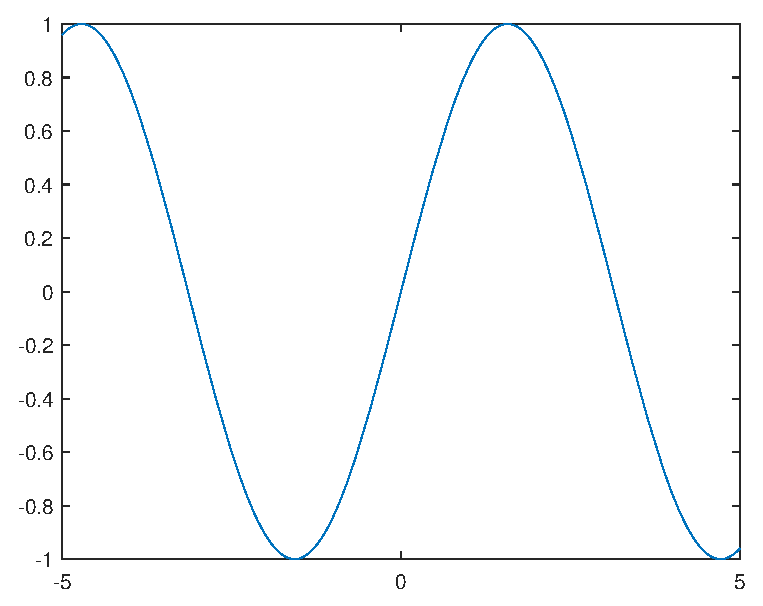
\includegraphics[width=0.5\linewidth]{image1}
\caption{图的描述.} \label{fig:A}
\end{figure}
\end{frame}

%------------------------------------------------

\begin{frame}
\frametitle{两图并排}
\begin{figure}[htb]
\centering
\begin{minipage}{0.48\linewidth}
\centering
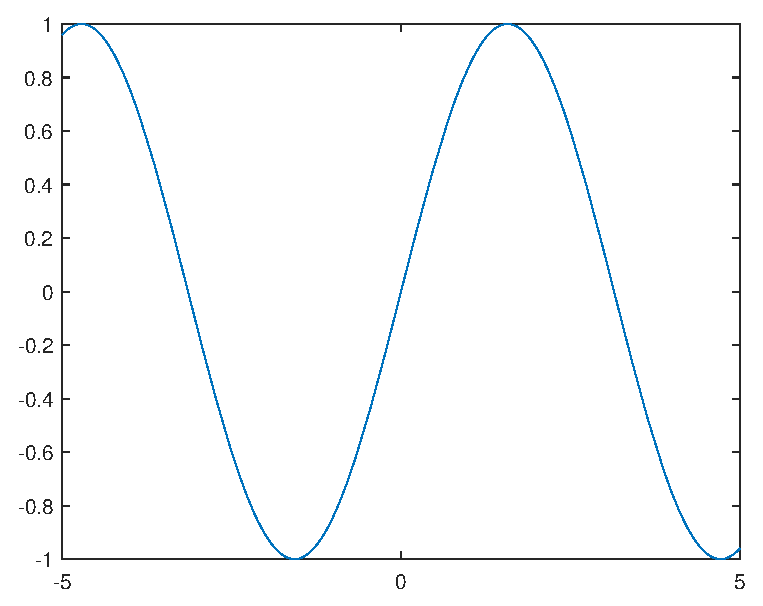
\includegraphics[width=\linewidth]{image1}
\caption{图~1~的描述.}
\end{minipage}\hfill
\begin{minipage}{0.48\linewidth}
\centering
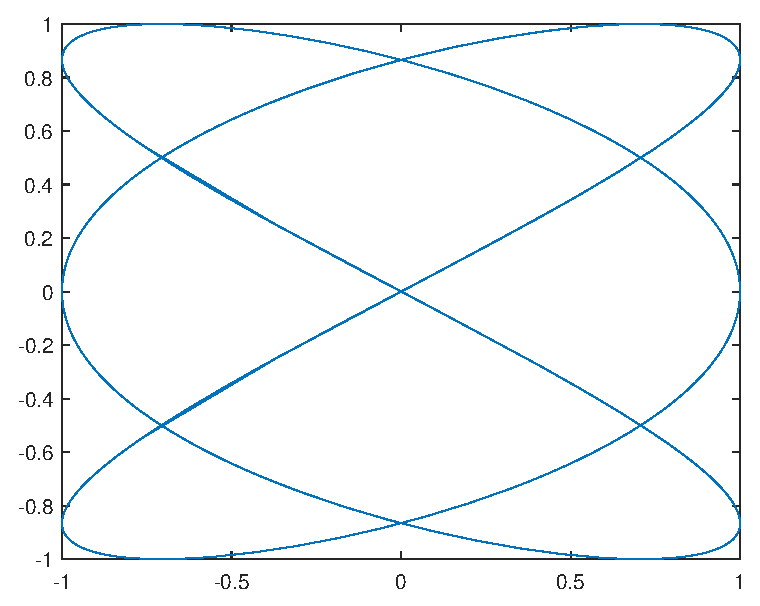
\includegraphics[width=\linewidth]{image2}
\caption{图~2~的描述.}
\end{minipage}
\end{figure}
\end{frame}

%------------------------------------------------
%\section{总结与展望}
%------------------------------------------------

\begin{frame}[fragile] % Need to use the fragile option when verbatim is used in the slide
\frametitle{Citation}
An example of the \verb|\cite| command to cite within the presentation:\\~

This statement requires citation \cite{Smith2012}. \\~

文献引用示例 \cite{LiLiu1997}, 可以修改引用文献样式.
\end{frame}

%------------------------------------------------

\begin{frame}
\frametitle{References}
\footnotesize{
\begin{thebibliography}{99} % Beamer does not support BibTeX so references must be inserted manually as below
\bibitem[Smith, 2012]{Smith2012} John Smith, Title of the publication, \emph{Journal Name}, 12(3):45--678, 2012.
\bibitem[李荣华, 1997]{LiLiu1997} 李荣华, 刘播. 微分方程数值解法. 东南大学出版社, 1997.
\end{thebibliography}
}
\end{frame}


%------------------------------------------------


%\setbeamertemplate{background canvas}[vertical shading][bottom=white,top=structure.fg!25]
%\setbeamertemplate{headline}{}
\begin{frame}
%\sffamily
\begin{center}
\HUGE \textcolor[RGB]{165,3,3}{谢\quad 谢! \\[8pt]
Thank you!}
\end{center}
\end{frame}


%------------------------------------------------


\end{document}

